\section{CAD Models and FEM Simulations}

\subsection{CAD Models}

CAD models were designed using SolidWorks\textsuperscript{\textregistered}. According to numerical models proposed for analysis, they are presented as follows.

\subsubsection{Top plate}

Figure \ref{CADTopPlate} presents CAD model for top plate which consists of a drop-shaped plane surface. Dimensions are specified in Figure \ref{PlateDimensions}.

As it was mentioned, simple models are pursued and hence, fan bracing, harmonic bars, bridge and sound hole reinforcement are not considered. These parts of the bandola, at low resonances, are expected to increase mass and stiffness without changing the shape modes.

\begin{figure}[h]
\centering
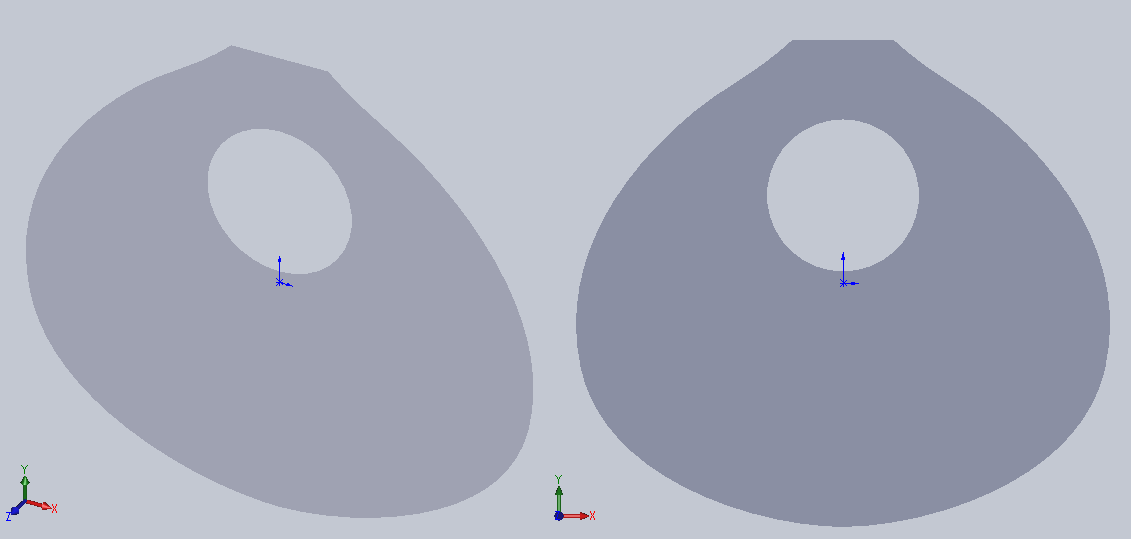
\includegraphics[height=7cm]{CADTopPlate.png}
\caption{CAD model for Top plate}
\label{CADTopPlate}
\end{figure}

\begin{figure}[h]
\centering
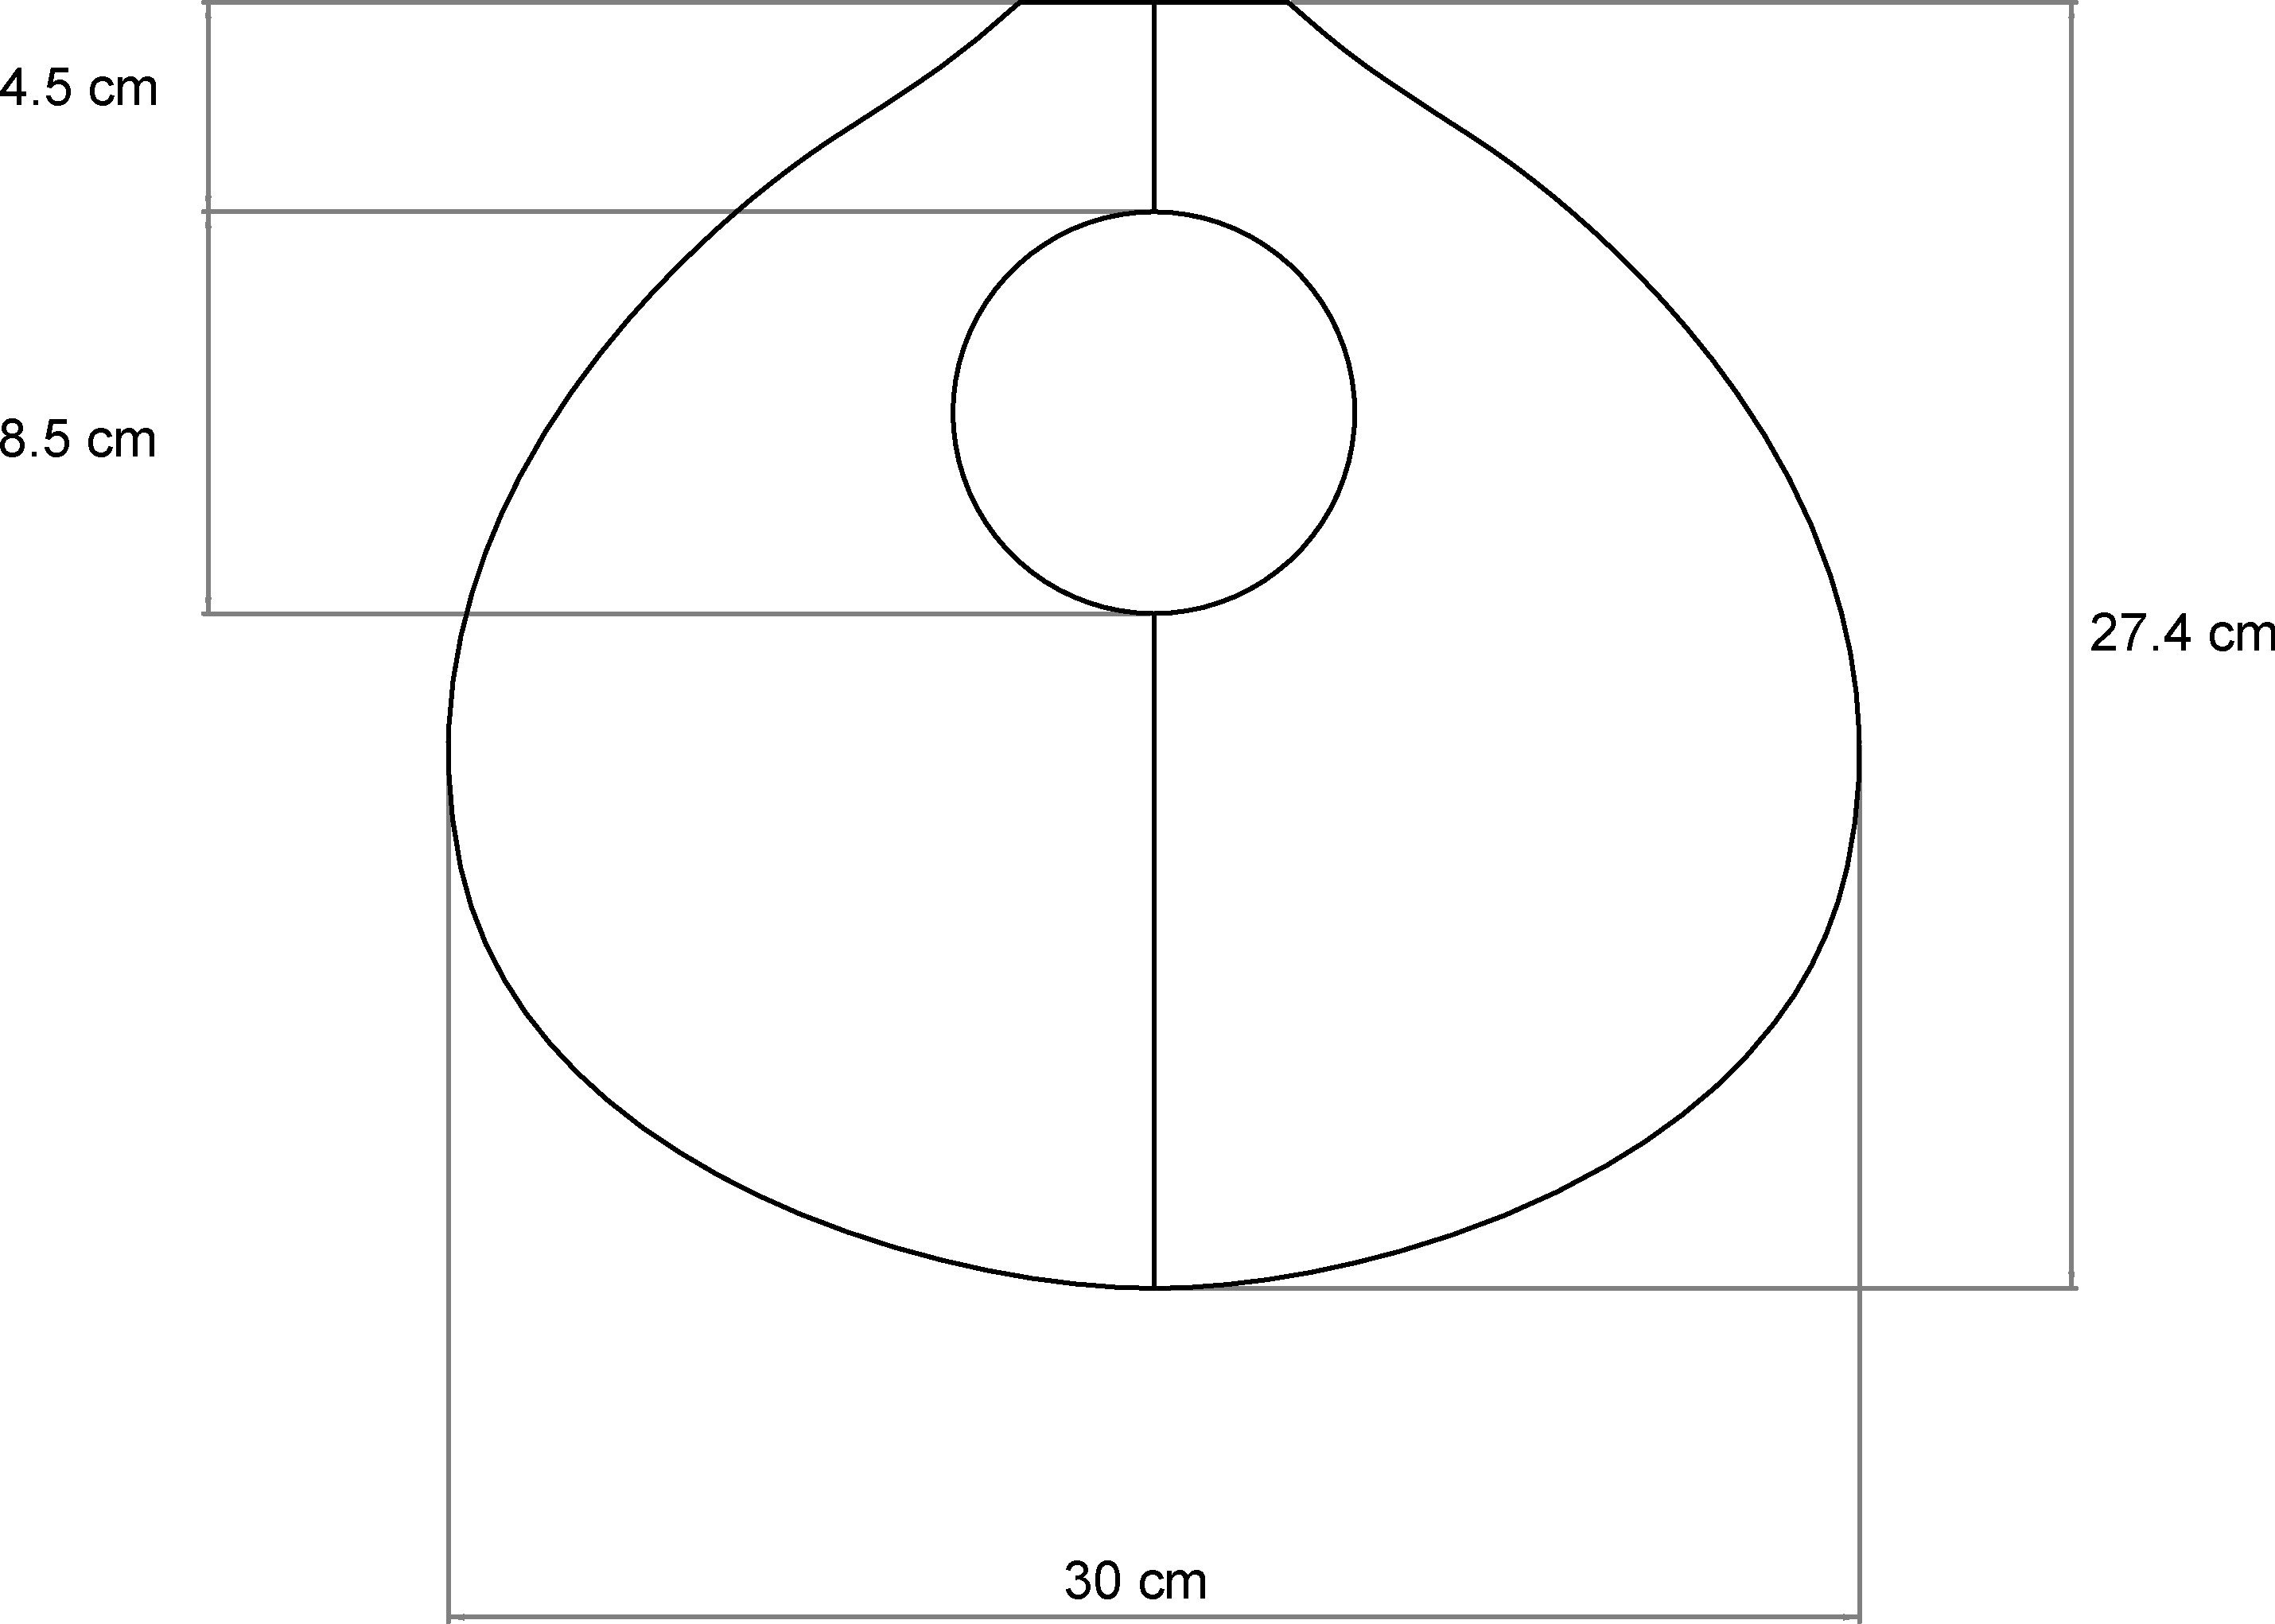
\includegraphics[height=7cm]{bandolaFrontarea.pdf}
\caption{Dimensions of modelled plates}
\label{PlateDimensions}
\end{figure}

\subsubsection{Back Plate}

For the same reasons as for top plate, reinforcement bars are not consider into the model. Figure \ref{CADBackPlate} presents CAD model for back plate which also consists of a drop-shaped plane surface. Dimensions are the same for top plate. 

\begin{figure}[h]
\centering
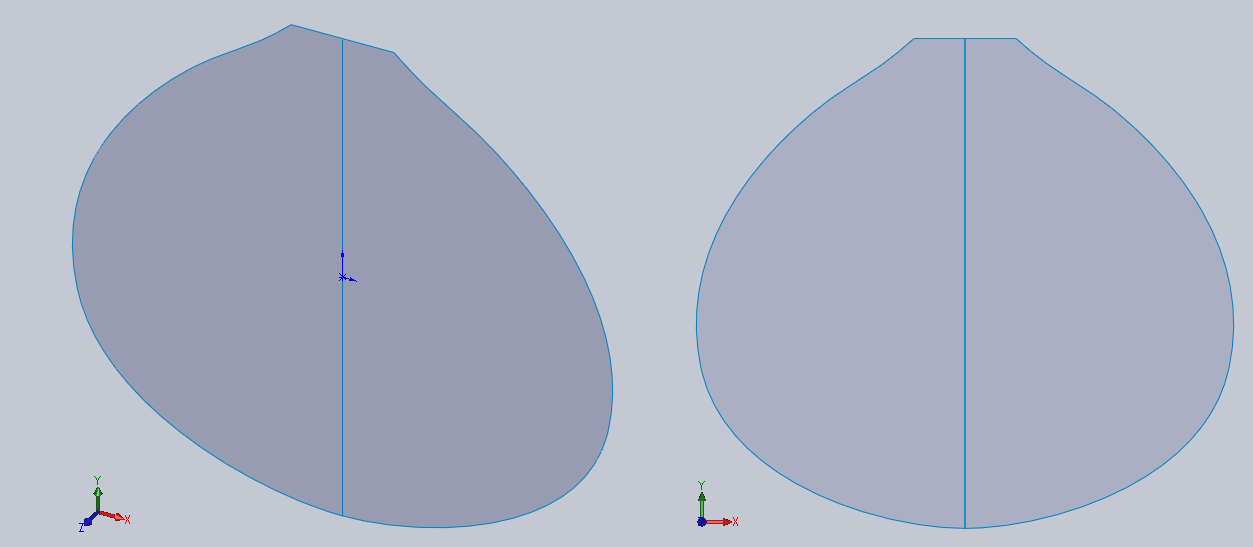
\includegraphics[height=6.5cm]{CADBackPlate.png}
\caption{CAD model for Back plate}
\label{CADBackPlate}
\end{figure}

\subsubsection{Enclosed air and coupled systems }

It was stated that the air inside the cavity vibrates at the first mode almost as a Helmholtz resonator. This assumption is not so simple because of the geometry of the instrument and also because the cavity walls are not completely rigid. Additionally, the concept of "length of the neck" does not refer exactly to a length determined by either end of the neck. In guitars, for example, it could be thought that the length of the plug of the air is given by top plate thickness, however, practice have shown that an extra volume both inside and outside moves with the air in the neck due to the inertia of the oscillating piston when it gets to its original position. This event is called the \emph{end effect} and the correction that should be applied in order to consider it is related to and of similar size to the diameter of the hole, so the mass of air is substantial. Applying the the correction used for guitars, the effective length of the "plug" of air of the bandola will be about 1.7 times the radius of the hole.

%which is given by top plate thickness (3mm).
The CAD model of enclosed air should represent the enclosed volume of air together with the effective length of the resonator's neck. The model presented in Figure \ref{CADBody} could represent not only the above ideas, but also the complete body, formed by surface planes for plates and enclosed volume of air, which is useful for coupling the systems. The ribs have a depth of 10cm as specified.

\begin{figure}[h]
\centering
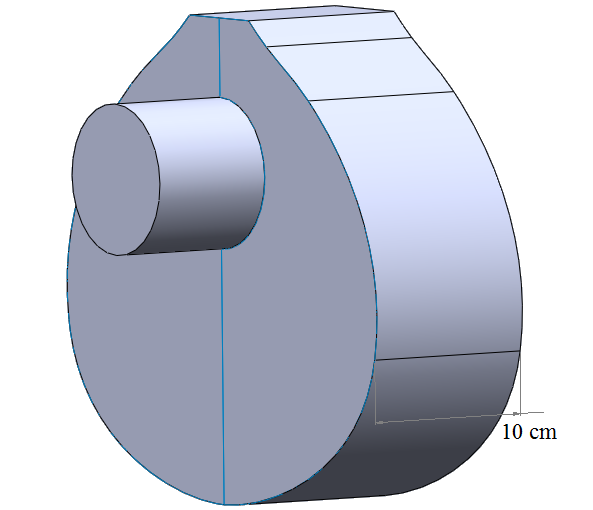
\includegraphics[height=9cm]{CADBody.png}
\caption{CAD model for Bandola's resonance box}
\label{CADBody}
\end{figure}

\subsection{Considerations for FEM Simulations}

Simulations were executed using the commercial software ANSYS\textsuperscript{\textregistered}. The elements in ANSYS\textsuperscript{\textregistered} library, used for meshing the plates and air, are presented as follows.

\subsubsection{Element SHELL281 for plates}

The analysis of plates was performed using the element SHELL281 whose formulation is based on the Mindlin-Reissner theory and hence, it is suitable for the analysis of thin to moderately-thick shell structures \cite{ANSYS}. The element is defined by shell section information and by eight nodes (I, J, K, L, M, N, O and P) with six degrees of freedom at each node: translations in the $x$, $y$, and $z$ axes, and rotations about the$x$, $y$, and $z$-axes. 

Figure \ref{Shell281} shows the geometry, node locations and the element coordinate system for this element. A triangular-shaped element may be formed by defining the same node number for nodes K, L and O.

\begin{figure}[h]
\centering
\includegraphics[height=5cm]{Shell281.png}
\caption{Geometry of element SHELL281 used for meshing the plates}
\label{Shell281}
\end{figure}

A mesh for the top plate using SHELL281 is presented in Figure \ref{TopPlateMesh}.

\begin{figure}[h]
\centering
\includegraphics[height=9cm]{TopPlateMesh.png}
\caption{The Top plate meshed with the element SHELL281}
\label{TopPlateMesh}
\end{figure}

\subsubsection{Element FLUID220 for air}

The element FLUID220 was used for meshing the air. This is a 3-D 20-node solid element that exhibits quadratic displacement behavior and is used for modeling the fluid medium and the interface in fluid/structure interaction problems \cite{ANSYS}. 

The element formulation is based on governing equation for acoustics, namely the 3-D wave equation, and also takes into account the coupling of acoustic pressure and structural motion at the interface. The element node has four degrees of freedom per node: translations in $x$, $y$ and $z$ directions, and pressure. The displacements are only applicable at nodes that are on the interface.

Figure \ref{Fluid220} shows the geometry, node locations and the coordinate system for this element.

\begin{figure}[h]
\centering
\includegraphics[height=6cm]{Fluid220.png}
\caption{Geometry of element FLUID220 used for meshing the air}
\label{Fluid220}
\end{figure}

A mesh for enclosed air using FLUID220 is presented in Figure \ref{AirMesh}.

\begin{figure}[h]
\centering
\includegraphics[height=10cm]{AirMesh.png}
\caption{The enclosed air meshed with the element FLUID220}
\label{AirMesh}
\end{figure}
